\chapter{Conception de la plateforme}

\section{Introduction}

L'objectif de ce travail, en premier lieu, est d'avoir un ensemble de données
composé d'images d'environnement avec un certain nombre de distances qui
représentent  les écarts respectifs entre la position de l'appareil permettant
de prendre chaque image et les obstacles qui sont y visibles.

Afin d'atteindre ce but nous avons vu la nécessité de fabriquer une machine mobile
permettant l'acquisition de ces données d'une manière automatique. La machine que
nous avons réalisé nous facilite la tâche et accélère énormément le rythme du travail.
De ce fait, nous pouvons obtenir une quantité importante de données dans un temps
réduit.

Cette machine possède une capacité limitée de navigation automatique, mais
elle peut être télécommandée par un ordinateur à travers une connexion sans fil
entre le programme qui s'exécute sur l'ordinateur et les programmes qui ordonnent
la machine. L'ensemble de ces programmes avec le matériel forment un système
qui a pour rôle de collecter les données nécessaires pour l'étape de
l'apprentissage automatique.

Le système est composé d'une partie matérielle et d'une autre logicielle. Chaque
partie sera présentée à part en montrant les détails de son fonctionnement.

\section{La partie matérielle}

La construction physique du robot est composée d'une carcasse et de plusieurs
parties électroniques, chaque partie offrant au moins une fonctionnalité
élémentaire. Les parties principales sont :

\begin{itemize}
  \item quatre moteurs de courant continu,
  \item un pilote de moteurs \keyword{L298N},
  \item des capteurs ultrasoniques \keyword{HC-S04},
  \item un moteur servo \keyword{TowerPro SG90},
  \item un capteur de température (et d'humidité) \keyword{DHT22},
  \item un microcontrôleur \keyword{Arduino Mega 2560},
  \item un appareil équipé du système d'exploitation \keyword{Android},
  disposant d'une camera RGB et d'un port USB qui permet la connexion en série
  (dans notre cas, nous avons utilisé un téléphone \keyword{Samsung Galaxy Note 2})
  \item une source d'alimentation électrique qui peut fournir une intensité de
  courant suffisante pour faire fonctionner les moteurs et les capteurs (nous
  avons utilisé une banque d'alimentation électrique combinée avec des piles).
\end{itemize}

\subsection{Le pilotage des moteurs}

Un moteur de courant continu tourne dans une seule direction à la fois. Cette
direction est déterminée par le sens du courant traversant la bobine interne
du moteur. La direction de la rotation peut être inversée seulement en inversant
le sens du courant électrique. De plus, l'intensité de ce courant détermine la
vitesse à laquelle ce moteur tourne.

\begin{figure}[h]
\begin{center}
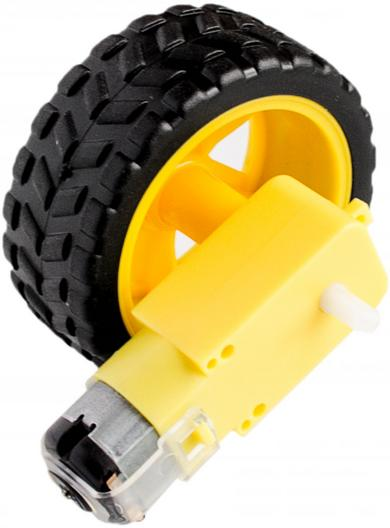
\includegraphics[width=0.2\textwidth]{DC_motor_wheel}
\caption{Le moteur de courant continu utilisé avec la roue}{}
\end{center}
\end{figure}

Pour pouvoir manipuler ces paramètres (le sens et la vitesse de la rotation), il
faut utiliser un pilote de moteurs comme \keyword{L298N}. Ce module peut contrôler
deux moteurs indépendamment, chacun dans un sens et à une vitesse donnée. Cependant, il est
aussi capable de gérer plus de deux moteurs, à condition qu'ils soient distribués
en deux groupes de telle manière que tous les moteurs du même groupe fonctionnent
par les mêmes paramètres.

Dans ce travail, nous avons eu recours à quatres moteurs
(pour supporter le poids du véhicule), chaque paire étant considérée comme un
seul groupe et située dans un côté du véhicule (droite ou gauche).
Les moteurs d'un côté tournent toujours dans le même sens avec la même vitesse.
La variance du sens entre les deux côtés détermine le type de mouvement : si
tous les moteurs tournent dans le même sens, alors le robot avance ou recule
selon le sens de la rotation, et si les moteurs des différents côtés tournent dans
des sens différents, alors le robot tourne autour de lui-même.

\begin{figure}[h]
\begin{center}
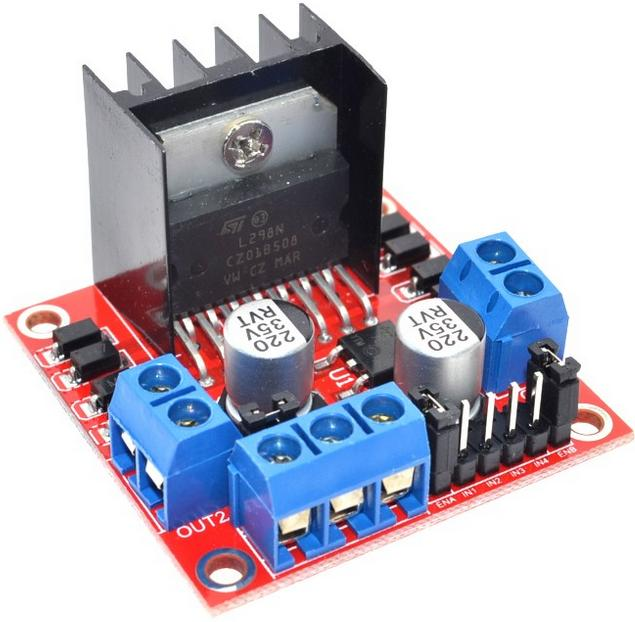
\includegraphics[width=0.3\textwidth]{L298N}
\caption{Le contrôleur de moteurs L298N}{}
\end{center}
\end{figure}

\subsection{La mesure de distances}

Les capteurs ultrasoniques sont des composants qui permettent l'envoi et la
réception du signal ultrasonique. En effet, ils sont utilisés pour le calcul
de la distance d'un objet. Pour ce faire, le capteur est commandé afin d'émettre
un signal dans une direction spécifiée. Si le signal ne frappe aucun objet avant de
s'affaiblir, il sera perdu et la distance ne pourra pas être calculée; sinon il
retournera au capteur à qui il notifiera le circuit commandant par la réception.
Par la suite, le circuit peut calculer la différence entre les instants d'émission
et de réception et utilise cette durée pour estimer la distance en connaissant
la vitesse du son dans l'air. La distance $d$ ($m/s$) est estimée par la formule suivante :

\begin{equation}
  d = t \times c \div 2,
\end{equation}

où $t$ est le temps écoulé en secondes entre l'envoi et la réception du signal,
et $c$ est la vitesse du son dans l'air sec et est approximée par la formule :

\begin{equation}
  c = 0.6 \times T + 331.4,
\end{equation}

avec $T$ la température de l'environnement en Celsius ($ ^\circ C$).

Afin de déterminer la température de l'air, nous avons utilisé le capteur
\keyword{DHT22} qui permet un relèvement de la température chaque $2$
secondes avec une haute précision (la marge d'erreur est seulement $\pm 0.5 ^\circ C$).

Ce capteur fonctionne en mode numérique. Il est activé seulement quand il reçoit
un signal approprié. Il renvoie le résultat à travers le même port au circuit
instantanément après avoir pris les mesures nécessaires.

\begin{figure}[h]
\begin{center}
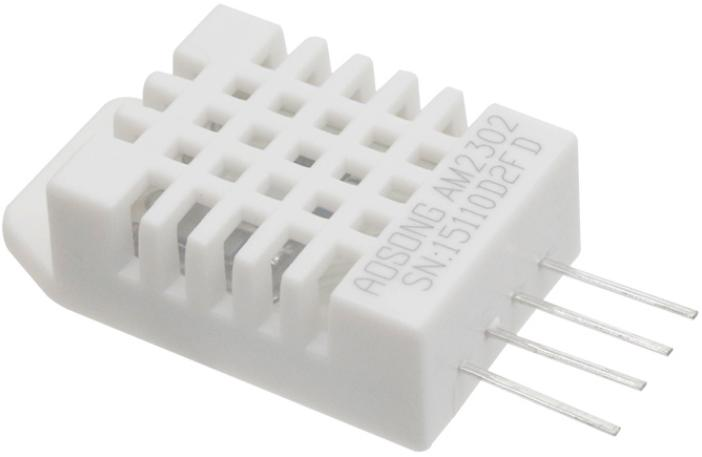
\includegraphics[width=0.25\textwidth]{DHT22}
\caption{Le capteur de la température DHT22}{}
\end{center}
\end{figure}

En outre, les capteurs d'ultrason opèrent sur une seule direction à la fois. Si
nous voulons avoir un ensemble de distances pour les différents obstacles éventuels
visibles dans le champ de vision du robot, nous avons besoin de plusieurs capteurs.

Mieux encore, on peut n'en utiliser qu'un seul et le faire tourner sous plusieurs
angles afin de couvrir la zone de vision.
Pour cela, il faut monter le capteur ultrasonique sur le bras d'un \keyword{servomoteur}.
Ces moteurs ont la capacité de déplacer leur bras par des angles exacts compris
généralement entre $0^\circ$ et $180^\circ$. Le circuit de contrôle envoie l'angle
d'inclinaison du bras au servomoteur qui effectue cette opération mécanique rapidement.
Nous avons utilisé le servomoteur \keyword{TowerPro SG90} pour cette tâche.

\begin{figure}[h]
\begin{center}
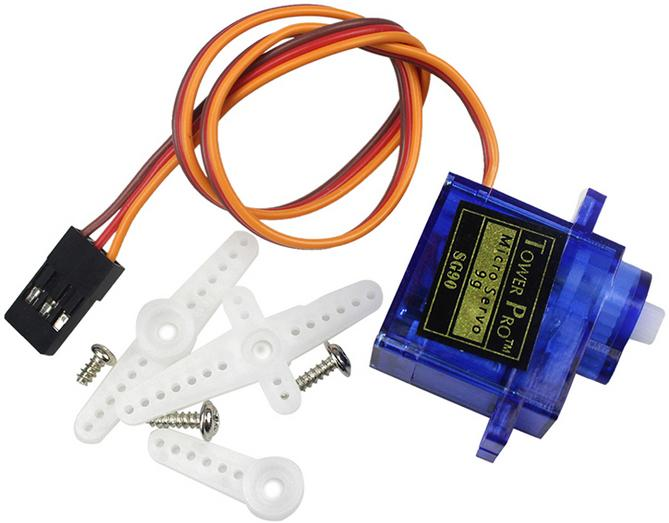
\includegraphics[width=0.3\textwidth]{SG90}
\caption{Le servomoteur TowerPro SG90}{}
\end{center}
\end{figure}
